% Sentinel: Utkrishta 2026, Challenge 2. The required 10-slide deck, written to be read on its own:
% every chart has a "How to read" line and most slides end with what it means.
% Build:  latexmk -xelatex sentinel.tex     Figures: python scripts/deck_figures.py
% Export: python scripts/export_pptx.py     (-> presentation/Sentinel.pdf + Sentinel.pptx)
% The earlier, more technical version is in old/sentinel_technical.tex.
\documentclass[aspectratio=169, 10pt]{beamer}
% Shared look for sentinel.tex (10 slides) and backup.tex (Q&A backup).
% Build: latexmk -xelatex sentinel.tex   (XeLaTeX: Fira Sans / Fira Math from the TeX tree)
\usetheme[progressbar=frametitle, numbering=fraction, titleformat frame=regular,
          sectionpage=none, block=fill]{metropolis}

\usepackage{fontspec}
\usepackage{unicode-math}
\setsansfont{FiraSans}[Extension=.otf, UprightFont=*-Book, BoldFont=*-SemiBold,
                       ItalicFont=*-BookItalic, BoldItalicFont=*-SemiBoldItalic]
\setmonofont{FiraMono}[Extension=.otf, UprightFont=*-Regular, BoldFont=*-Medium, Scale=0.9]
\setmathfont{FiraMath-Regular.otf}

\usepackage{booktabs}
\usepackage{array}
\usepackage{tikz}
\usetikzlibrary{arrows.meta, positioning, calc, decorations.pathreplacing}
\graphicspath{{figures/}}

% palette: the same colours as every figure
\definecolor{ink}{HTML}{0B0B0B}
\definecolor{ink2}{HTML}{52514E}
\definecolor{muted}{HTML}{898781}
\definecolor{line}{HTML}{C3C2B7}
\definecolor{soft}{HTML}{F3F2EE}
\definecolor{slate}{HTML}{1E2A35}
\definecolor{sblue}{HTML}{2A78D6}
\definecolor{sorange}{HTML}{EB6834}
\definecolor{sred}{HTML}{D03B3B}
\definecolor{winfill}{HTML}{E4E3DF}

\setbeamersize{text margin left=6mm, text margin right=6mm}
\hyphenpenalty=10000\exhyphenpenalty=10000   % no hyphenated words on slides
\setbeamercolor{normal text}{fg=ink, bg=white}
\setbeamercolor{frametitle}{bg=slate, fg=white}
\setbeamercolor{progress bar}{fg=sorange, bg=slate}
\setbeamercolor{alerted text}{fg=sorange}
\setbeamercolor{frame numbering}{fg=muted}
\setbeamercolor{footline}{fg=muted}
\setbeamerfont{frametitle}{size=\large, series=\bfseries}
\setbeamerfont{frame footer}{size=\tiny}
\setbeamerfont{page number in head/foot}{size=\tiny}
\setbeamertemplate{frame footer}{Sentinel \,·\, Utkrishta 2026 \,·\, Challenge 2}

% team details: edit these two lines
\newcommand{\teamname}{if/elif/else}
\newcommand{\members}{Aarohi Gattewar \,·\, Phalak Mehta \,·\, Harshit Singh}

% building blocks
\newcommand{\hl}[1]{\textcolor{sblue}{\bfseries #1}}
\newcommand{\figcap}[1]{\par\vspace{0.6mm}{\scriptsize\color{ink2}#1\par}}
\newcommand{\head}[1]{{\small\bfseries #1\par}\vspace{0.8mm}}
\newcommand{\alarmmark}[1][sred]{\tikz[baseline=-0.15ex]\fill[#1] (0,0.75ex) -- (1ex,0.75ex) -- (0.5ex,-0.15ex) -- cycle;}
% a row of 4 headline numbers on one baseline: \kpirow{n1}{l1}{n2}{l2}{n3}{l3}{n4}{l4}
\newcommand{\kpinum}[1]{{\fontsize{21}{23}\selectfont\bfseries\color{sblue}#1}}
\newcommand{\kpilab}[1]{{\scriptsize\color{ink2}#1}}
\newcommand{\kpicell}[1]{\makebox[0.25\linewidth][l]{\kpinum{#1}}}
\newcommand{\kpilabcell}[1]{\makebox[0.25\linewidth][l]{\kpilab{#1}}}   % labels are one line each
\newcommand{\kpirow}[8]{%
  {\noindent\kpicell{#1}\kpicell{#3}\kpicell{#5}\kpicell{#7}\par\vspace{-2.6mm}%
   \noindent\kpilabcell{#2}\kpilabcell{#4}\kpilabcell{#6}\kpilabcell{#8}\par}}
\newcommand{\chip}[1]{\tikz[baseline=(c.base)]\node[fill=soft, rounded corners=5pt, inner xsep=5pt,
  inner ysep=2.5pt, font=\scriptsize, text=ink2] (c) {#1};}
\newcommand{\need}[3]{%
  \begin{tikzpicture}[baseline=(n.north)]
    \node[circle, fill=sblue, text=white, minimum size=5.5mm, inner sep=0pt, font=\small\bfseries] (n) {#1};
  \end{tikzpicture}\hspace{2.5mm}%
  \begin{minipage}[t]{5.55cm}\raggedright\vspace{-1.6mm}{\bfseries #2}\\[0.5mm]{\footnotesize\color{ink2}#3}\end{minipage}}
\newcommand{\evidence}[3]{% #1 colour, #2 header, #3 sentence
  \begin{tikzpicture}
    \node[fill=soft, text width=5.5cm, inner xsep=5pt, inner ysep=4pt, align=left, font=\scriptsize] (e)
      {{\bfseries\color{#1}#2}\\[1pt]{\color{ink}#3}};
    \draw[#1, line width=2pt] (e.north west) -- (e.south west);
  \end{tikzpicture}}
% self-explanatory deck: a "How to read" line under each chart, a summary box per slide
\newcommand{\howto}[1]{\figcap{\textbf{\color{ink}How to read.} #1}}
\newcommand{\abox}[3]{% #1 width, #2 title, #3 text
  \begin{tikzpicture}[baseline=(a.north)]
    \node[fill=soft, text width=#1, inner xsep=6pt, inner ysep=5pt, align=left, font=\scriptsize] (a)
      {{\footnotesize\bfseries\color{sblue}#2}\\[2pt]{\color{ink}#3}};
  \end{tikzpicture}}
\newcommand{\ev}[2]{% full-width evidence card: #1 header, #2 the sentence Sentinel wrote
  \begin{tikzpicture}
    \node[fill=soft, text width=\dimexpr\linewidth-12pt\relax, inner xsep=5pt, inner ysep=3pt, align=left,
          font=\scriptsize] (e) {{\bfseries\color{sblue}#1}\\[1pt]{\color{ink}#2}};
    \draw[sblue, line width=2pt] (e.north west) -- (e.south west);
  \end{tikzpicture}}
\newcolumntype{L}[1]{>{\raggedright\arraybackslash}p{#1}}
\newcommand{\bandnote}[1]{%
  \begin{tikzpicture}
    \node[fill=soft, text width=\dimexpr\linewidth-10pt\relax, inner xsep=5pt, inner ysep=4pt,
          align=left, font=\scriptsize] (b) {#1};
    \draw[sorange, line width=2pt] (b.north west) -- (b.south west);
  \end{tikzpicture}}


\begin{document}

% =================================================================== 1. title + one-line summary
\begin{frame}[plain]
  \vspace*{0.5mm}% (a brace group right after \begin{frame} would be read as the frame title)
  {\scriptsize\color{muted}UTKRISHTA 2026 \,·\, CHALLENGE 2 \,·\, ADAPTIVE TIME-SERIES ANOMALY DETECTION
   \hfill TEAM \textcolor{ink}{\bfseries\teamname}}\par\vspace{3mm}
  {\fontsize{28}{30}\selectfont\bfseries Sentinel}\hspace{3mm}%
  {\large\color{ink2}a live anomaly detector that explains every alarm}\par\vspace{2.5mm}
  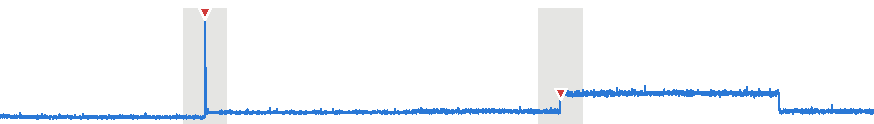
\includegraphics{hero}\par\vspace{-0.8mm}
  \howto{a real database server's CPU, streamed one value at a time. Grey bands: the two moments
    experts labelled as anomalies. \alarmmark\ Sentinel's alarms: both anomalies caught, nothing else flagged.}
  \vspace{3.5mm}
  \abox{4.35cm}{The problem}{Machines and apps send a number every few minutes. Flag the truly abnormal
    moments \textbf{live}, without false alarms, and say \textbf{why}.}\hfill
  \abox{4.35cm}{Our solution}{Five watchers score each new value; a \textbf{rarity meter} learned per signal
    turns it into a probability. Alarm only if rarer than \textbf{1 in 100,000}.}\hfill
  \abox{4.35cm}{The result}{All 58 benchmark signals: \textbf{event-F1 0.594}, the \textbf{best of 8 methods}
    tested (next: 0.316), \textbf{39} false alarms in 365,558 values, \textbf{61\,µs} per value.}
  \vfill
  {\small\bfseries\teamname}\hspace{3mm}{\small\color{ink2}\members}\hfill
  {\scriptsize\color{muted}Every chart in this deck has a “How to read” note.}
  \vspace*{0.5mm}
\end{frame}

% =================================================================== 2. problem
\begin{frame}{The problem: catch real failures in live data, without crying wolf}
  \begin{columns}[T,onlytextwidth]
    \column{0.5\textwidth}
      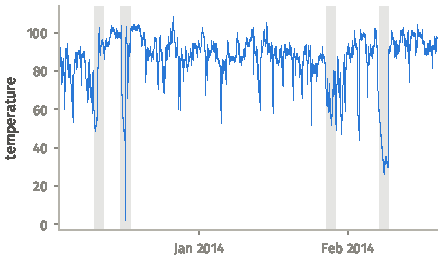
\includegraphics[width=\linewidth]{machine}
      \howto{the temperature inside an industrial machine over three months. Grey bands: the 4 moments
        experts labelled as anomalies, around a known system failure. A good detector raises an alarm
        inside each band and nowhere else.}
    \column{0.47\textwidth}
      \head{What the challenge asks}
      {\scriptsize\setlength{\tabcolsep}{0pt}
      \begin{tabular}{@{}L{1.5cm}L{5.4cm}@{}}
        \textbf{Input}     & a stream of values, one at a time. Decide at once, never look ahead.\\[1.2mm]
        \textbf{Output}    & for every value: an anomaly score, a NORMAL / ANOMALOUS label, and
                             evidence explaining each alarm.\\[1.2mm]
        \textbf{Scored by} & event-F1 (main score), precision, recall, detection delay, runtime.\\
      \end{tabular}\par}
      \vspace{3mm}
      \head{Two ways to fail}
      {\scriptsize\raggedright
      \textcolor{sorange}{\bfseries Stay quiet:} the early warning is missed and the failure becomes an outage.\\[0.8mm]
      \textcolor{sorange}{\bfseries Cry wolf:} too many alarms, so people stop listening and miss the real one.\par}
      \vspace{3mm}
      \head{Why it matters}
      {\scriptsize\raggedright Cloud servers, factories, online ads, city traffic, social media: a missed
      failure costs money, a noisy alarm costs trust.\par}
  \end{columns}
  \vfill
  \bandnote{\textbf{Our goal.} Alarm only when a value is truly unusual \emph{for its own signal}, decide live,
    and explain every alarm in one sentence.}
\end{frame}

% =================================================================== 3. data, EDA, preprocessing
\begin{frame}{Why it is hard: every signal is different, and extremes are normal}
  \begin{columns}[T,onlytextwidth]
    \column{0.37\textwidth}
      \head{The data (Numenta benchmark)}
      {\scriptsize\setlength{\tabcolsep}{2.5pt}
      \begin{tabular}{@{}l r r r@{}}
        \toprule
        & signals & values & anomalies\\
        \midrule
        Twitter mentions  & 10 & 158,631 & 33\\
        Cloud servers     & 17 & 67,740  & 30\\
        Known failures    & 7  & 69,561  & 19\\
        Road traffic      & 7  & 15,664  & 14\\
        Online ad prices  & 6  & 9,610   & 14\\
        Synthetic         & 11 & 44,352  & 6\\
        \midrule
        \textbf{Total}    & \textbf{58} & \textbf{365,558} & \textbf{116}\\
        \bottomrule
      \end{tabular}\par}
      \vspace{2mm}
      \head{What the data taught us}
      {\scriptsize\raggedright
      \textbf{Extremes are normal:} 47 of 58 signals have heavy tails.\\[0.6mm]
      \textbf{Rhythm matters:} 18 signals repeat every day.\\[0.6mm]
      \textbf{Preprocessing:} none needed. No missing values; read in time order, unscaled.\par}
    \column{0.6\textwidth}
      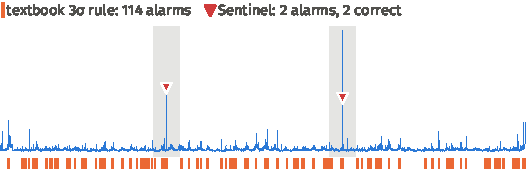
\includegraphics{sigma_rule}
      \howto{tweets about Facebook. Orange ticks: the textbook 3σ rule fires 114 times. \alarmmark\ Sentinel fires
        twice, both inside labelled anomalies (grey bands).}
      \vspace{1mm}
      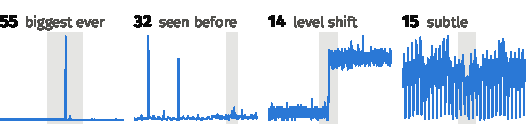
\includegraphics{types_strip}
      \howto{the 116 anomalies by type. “Seen before”: a bigger spike came earlier.}
  \end{columns}
  \vfill
  \bandnote{\textbf{What this means.} The 3σ rule raises \textbf{2,403 alarms for 116 real anomalies}, so
    Sentinel alarms on rarity instead.}
\end{frame}

% =================================================================== 4. system design
\begin{frame}{Our solution: five watchers ask one question, “how rare is this?”}
  \centering
  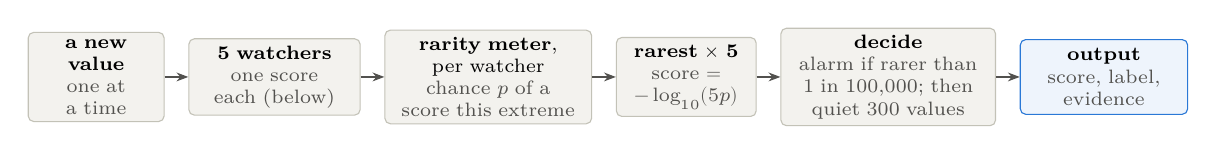
\begin{tikzpicture}[font=\scriptsize, >={Stealth[length=1.5mm]},
      n/.style={draw=line, fill=soft, rounded corners=2pt, inner sep=2.5pt, align=center, minimum height=0.95cm},
      a/.style={->, draw=ink2, line width=0.45pt}]
    \node[n, text width=1.55cm] (a) {\textbf{a new value}\\{\color{ink2}one at a time}};
    \node[n, text width=2.0cm, right=3mm of a] (b) {\textbf{5 watchers}\\{\color{ink2}one score each (below)}};
    \node[n, text width=2.45cm, right=3mm of b] (c) {\textbf{rarity meter}, per watcher\\{\color{ink2}chance $p$ of a score this extreme}};
    \node[n, text width=1.6cm, right=3mm of c] (d) {\textbf{rarest $\times$ 5}\\{\color{ink2}score $= -\log_{10}(5p)$}};
    \node[n, text width=2.55cm, right=3mm of d] (e) {\textbf{decide}\\{\color{ink2}alarm if rarer than 1 in 100,000; then quiet 300 values}};
    \node[n, text width=1.95cm, right=3mm of e, fill=sblue!8, draw=sblue] (f) {\textbf{output}\\{\color{ink2}score, label, evidence}};
    \foreach \u/\v in {a/b, b/c, c/d, d/e, e/f} \draw[a] (\u) -- (\v);
  \end{tikzpicture}

  \vspace{2.5mm}
  \raggedright
  {\scriptsize\setlength{\tabcolsep}{3pt}\renewcommand{\arraystretch}{1.05}
  \begin{tabular}{@{}L{1.55cm} L{4.35cm} L{1.5cm} L{5.4cm} r@{}}
    \toprule
    watcher & what it measures, for every value & looks back (past only) & what it catches, with a real alarm it wrote & alarms (real)\\
    \midrule
    \textbf{Spike} & distance from its running average, in running spreads (outliers clipped)
      & ≈\,50 values & spikes and dips: \emph{“Value 50.00 is 99.4 scales above the learned baseline 0.32”} & 43 (30)\\[0.6mm]
    \textbf{Routine} & the same, for the change since a day earlier; daily signals only & one day &
      a normal value at the wrong time: \emph{“Value 40.00 breaks the repeating pattern”} & 7 (6)\\[0.6mm]
    \textbf{New level} & a fast average minus a slow average, in spreads & 10 vs.\ 200 & a level that moves and stays:
      \emph{“recent mean 6.40 vs baseline 0.43”} (tweets) & 24 (12)\\[0.6mm]
    \textbf{Jitter} & recent step size divided by long-run step size (log) & 10 vs.\ 200 & noise bursts or a frozen
      sensor: \emph{“Signal went unusually flat: volatility is 0.21x its baseline”} & 9 (3)\\[0.6mm]
    \textbf{New shape} & distance from the last 8 values to their closest match in the past 2,000 & 2,000 values &
      a never-seen pattern (repeats stop alarming): \emph{“closest past match differs by 0.27 per point”} & 23 (16)\\
    \bottomrule
  \end{tabular}\par}
  \figcap{\textbf{How to read.} One row per watcher. “Alarms (real)”: of the 106 final alarms, how many it raised and how many
    were real. Each value is scored \emph{before} the watchers learn from it.}
\end{frame}

% =================================================================== 5. core algorithm: adaptive threshold
\begin{frame}{The key idea: alarm on rarity, not on a fixed number}
  \begin{columns}[T,onlytextwidth]
    \column{0.52\textwidth}
      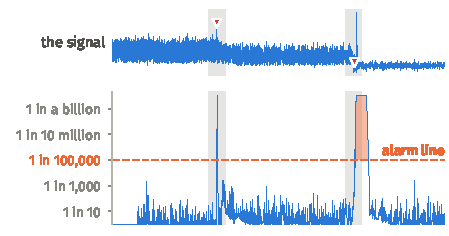
\includegraphics{score_chart}
      \howto{top, a cloud server's CPU. Bottom, each value's rarity \emph{for this signal}, as “1 in N”. Only
        values above the dashed line alarm: two here, both real.}
      \vspace{1.2mm}
      {\scriptsize\raggedright\textbf{How the rarity meter works.} Each watcher fits a curve (extreme-value theory)
      to its largest 5\% of past scores; it gives $p$, the chance of a score this large.
      Score $= -\log_{10}(5 \cdot \min p)$; alarm if $\geq 5$.\par}
      \vspace{1.2mm}
      {\scriptsize\raggedright\textbf{\color{sorange}Why this model.} No training set: it learns each signal from its
      first 300 values. Unlike an autoencoder, it keeps adapting and explains every alarm.\par}
    \column{0.45\textwidth}
      \head{Two fixes we made this round}
      {\scriptsize\raggedright\textbf{\color{sorange}Fix 1 · Don't jump to conclusions.} After warm-up a watcher has
      seen only about 12 extremes; its curve was often far too heavy (“huge values are normal”), so obvious spikes
      could not alarm. Now a heavy tail needs real evidence.\par}
      \vspace{1mm}
      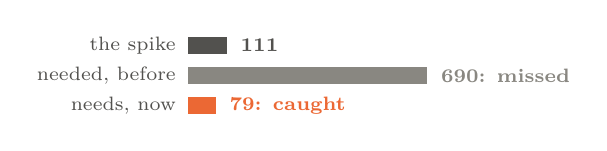
\begin{tikzpicture}[font=\scriptsize, x=0.0044cm]
        \foreach \y/\lab/\v/\col/\txt in {0/{the spike}/111/ink2/{111}, -0.38/{needed, before}/690/muted/{690: missed},
                                         -0.76/{needs, now}/79/sorange/{79: caught}} {
          \node[anchor=east, text=ink2] at (0,\y) {\lab};
          \fill[\col] (8,\y-0.11) rectangle (8+\v,\y+0.11);
          \node[anchor=west, text=\col, font=\scriptsize\bfseries] at (20+\v,\y) {\txt};
        }
      \end{tikzpicture}
      \figcap{A real spike in an hourly ad price. Biggest-ever spikes caught: \textbf{31 → 37}.}
      \vspace{2mm}
      {\scriptsize\raggedright\textbf{\color{sorange}Fix 2 · Accept a new normal.} If a problem is still on after the
      300-value quiet period, the signal has changed: Sentinel re-learns normal instead of alarming again and again.\par}
      \vspace{1mm}
      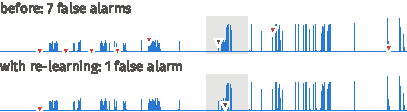
\includegraphics[width=\linewidth]{relearn_strip}
      \figcap{Disk writes: false alarms \textbf{7 → 1}, no anomaly lost.}
  \end{columns}
\end{frame}

% =================================================================== 6. experiments
\begin{frame}{How we tuned it: one idea per run, kept only if the score went up}
  \begin{columns}[T,onlytextwidth]
    \column{0.49\textwidth}
      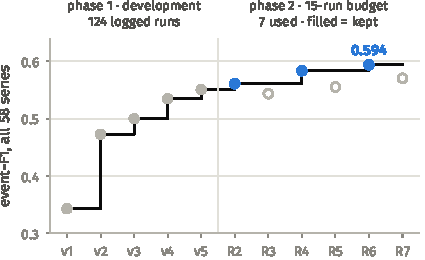
\includegraphics{trajectory}
      \howto{each dot is one full run on all 58 signals; the line is the best score so far. Grey: development
        versions v1 to v5. Blue: budgeted runs, filled if the idea was kept, hollow if dropped.}
    \column{0.48\textwidth}
      {\scriptsize\setlength{\tabcolsep}{3pt}
      \begin{tabular}{@{}c l r l@{}}
        \toprule
        run & what changed & event-F1 & decision\\
        \midrule
        1 & starting point (v5), reproduced     & 0.551 & reference\\
        2 & fix 1, light                        & 0.561 & \hl{kept}\\
        3 & fix 1, strong                       & 0.544 & {\color{muted}dropped}\\
        4 & + fix 2 (re-learning)               & 0.584 & \hl{kept}\\
        5 & shorter learning: 300 → 200 values  & 0.556 & {\color{muted}dropped}\\
        6 & fix 1, medium + re-learning         & \textbf{0.594} & \hl{kept, final}\\
        7 & fix 1, strong + re-learning         & 0.571 & {\color{muted}dropped}\\
        \bottomrule
      \end{tabular}\par}
      \vspace{3mm}
      \head{Search strategy}
      {\scriptsize\raggedright
      \textbf{Budget:} at most 15 runs; one run = all 58 signals, scored once.\\[0.7mm]
      \textbf{Think first:} ideas were tested on saved outputs for free; 7 were dropped without a run.\\[0.7mm]
      \textbf{One change per run,} its hypothesis written down before it started.\\[0.7mm]
      \textbf{Keep rule:} event-F1 must rise \emph{and} more categories must gain than lose.\par}
  \end{columns}
  \vfill
  \bandnote{\textbf{What this means.} 0.551 → \textbf{0.594} with 7 of the 15 runs (8 kept in reserve). Only
    global settings were changed, never one signal at a time.}
\end{frame}

% =================================================================== 7. evaluation
\begin{frame}{How we measure it: per incident, the way the challenge scores it}
  \begin{columns}[T,onlytextwidth]
    \column{0.5\textwidth}
      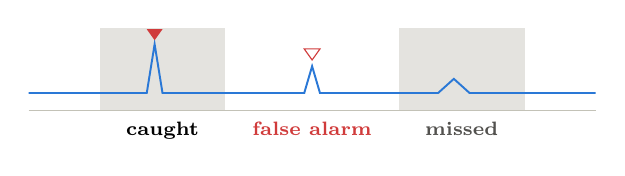
\begin{tikzpicture}[font=\scriptsize, x=1cm, y=1cm]
        \fill[winfill] (0.9,0) rectangle (2.5,1.05);
        \fill[winfill] (4.7,0) rectangle (6.3,1.05);
        \draw[line, line width=0.4pt] (0,0) -- (7.2,0);
        \draw[sblue, line width=0.7pt] (0,0.22) -- (1.5,0.22) -- (1.6,0.84) -- (1.7,0.22) -- (3.5,0.22)
          -- (3.6,0.56) -- (3.7,0.22) -- (5.2,0.22) -- (5.4,0.4) -- (5.6,0.22) -- (7.2,0.22);
        \fill[sred] (1.5,1.03) -- (1.7,1.03) -- (1.6,0.89) -- cycle;
        \draw[sred, fill=white] (3.5,0.78) -- (3.7,0.78) -- (3.6,0.64) -- cycle;
        \node[below] at (1.7,-0.02) {\textbf{caught}};
        \node[below, text=sred] at (3.6,-0.02) {\textbf{false alarm}};
        \node[below, text=ink2] at (5.5,-0.02) {\textbf{missed}};
      \end{tikzpicture}
      \howto{grey bands are labelled anomalies. Alarm in a band: caught. Alarm outside every band: false alarm.
        Band with no alarm: missed. One burst of alarms counts once.}
      \vspace{1mm}
      {\scriptsize\setlength{\tabcolsep}{2.5pt}
      \begin{tabular}{@{}l L{4.75cm} r@{}}
        \toprule
        metric & plain question & ours\\
        \midrule
        Precision & of our alarms, how many were real? & 0.63\\
        Recall    & of the real anomalies, how many were caught? & 0.56\\
        Event-F1  & both combined: the main score & \textbf{0.594}\\
        Delay     & first alarm minus labelled anomaly point & 0 steps\\
        \bottomrule
      \end{tabular}\par}
      \vspace{1.5mm}
      {\scriptsize\raggedright\textbf{Checks.} One setting for all signals · a category left out: still
      \textbf{0.594} · 5 clean signals: \textbf{0 alarms}.\par}
    \column{0.47\textwidth}
      {\scriptsize\setlength{\tabcolsep}{4pt}
      \begin{tabular}{@{}l r r r r@{}}
        \toprule
        category & anomalies & precision & recall & event-F1\\
        \midrule
        Synthetic           & 6  & 1.00 & 0.83 & 0.91\\
        Twitter mentions    & 33 & 0.57 & 0.76 & 0.65\\
        Known failures      & 19 & 0.52 & 0.63 & 0.57\\
        Cloud servers       & 30 & 0.67 & 0.47 & 0.55\\
        Online ad prices    & 14 & 1.00 & 0.36 & 0.53\\
        Road traffic        & 14 & 0.80 & 0.29 & 0.42\\
        \midrule
        \textbf{All}        & \textbf{116} & \textbf{0.63} & \textbf{0.56} & \textbf{0.594}\\
        \bottomrule
      \end{tabular}\par}
      \vspace{2mm}
      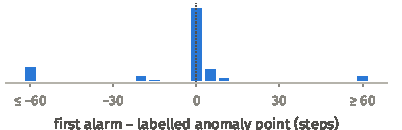
\includegraphics{delay_hist}
      \howto{first alarm relative to the labelled anomaly point (0). Median \textbf{0 steps}; 66\% within 10.}
  \end{columns}
  \vfill
  \bandnote{\textbf{What this means.} Right 2 times in 3 when it alarms, over half of all anomalies caught, on time.}
\end{frame}

% =================================================================== 8. results
\begin{frame}{Results: the best of all 8 methods, with 6 to 15 times fewer false alarms}
  \begin{columns}[T,onlytextwidth]
    \column{0.58\textwidth}
      {\scriptsize\setlength{\tabcolsep}{3.2pt}
      \begin{tabular}{@{}l r r r r r@{}}
        \toprule
        method & event-F1 & precision & recall & false alarms & µs/value\\
        \midrule
        \textbf{\color{sblue}Sentinel (ours)} & \textbf{0.594} & \textbf{0.63} & 0.56 & \textbf{39} & 61\\
        Temporal clustering  & 0.316 & 0.22 & 0.53 & 249 & 6\\
        Ensemble of all 6    & 0.280 & 0.18 & 0.65 & 419 & 221\\
        Autoencoder          & 0.272 & 0.18 & 0.60 & 390 & 140\\
        Local Outlier Factor & 0.260 & 0.16 & 0.62 & 457 & 13\\
        Isolation Forest     & 0.249 & 0.18 & 0.42 & 261 & 54\\
        One-Class SVM        & 0.235 & 0.14 & 0.68 & 594 & 8\\
        Rolling z-score      & 0.226 & 0.15 & 0.47 & 351 & 0.5\\
        \bottomrule
      \end{tabular}\par}
      \howto{every model family named in the problem statement, same data, same scoring, each learning from the
        first 300 values of every signal. Each got its \textbf{best threshold, chosen using the answers}; Sentinel uses
        one fixed setting. Sentinel: 65 of 116 anomalies caught; the others' higher recall costs 6 to 15× more false alarms.}
    \column{0.39\textwidth}
      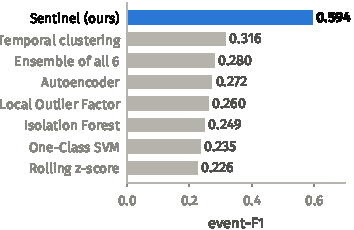
\includegraphics[width=\linewidth]{f1_bars}
  \end{columns}
  \vspace{1mm}
  {\small\bfseries Why 0.594 is a strong score\par}\vspace{-4mm}% the boxes hang from their top edge
  \abox{4.45cm}{1.9× the runner-up}{temporal clustering, even with its threshold tuned on the answers;
    2.3× the best standard method.}\hfill
  \abox{4.45cm}{Few alarms, mostly real}{one false alarm per 9,400 values, about one a month on a 5-minute
    signal.}\hfill
  \abox{4.45cm}{Why papers quote 0.9+}{they use “point adjustment”, where random alarms score 0.92 (0.16
    here).}
\end{frame}

% =================================================================== 9. demo
\begin{frame}{See it work: every alarm comes with a reason a person can read}
  \begin{columns}[T,onlytextwidth]
    \column{0.37\textwidth}
      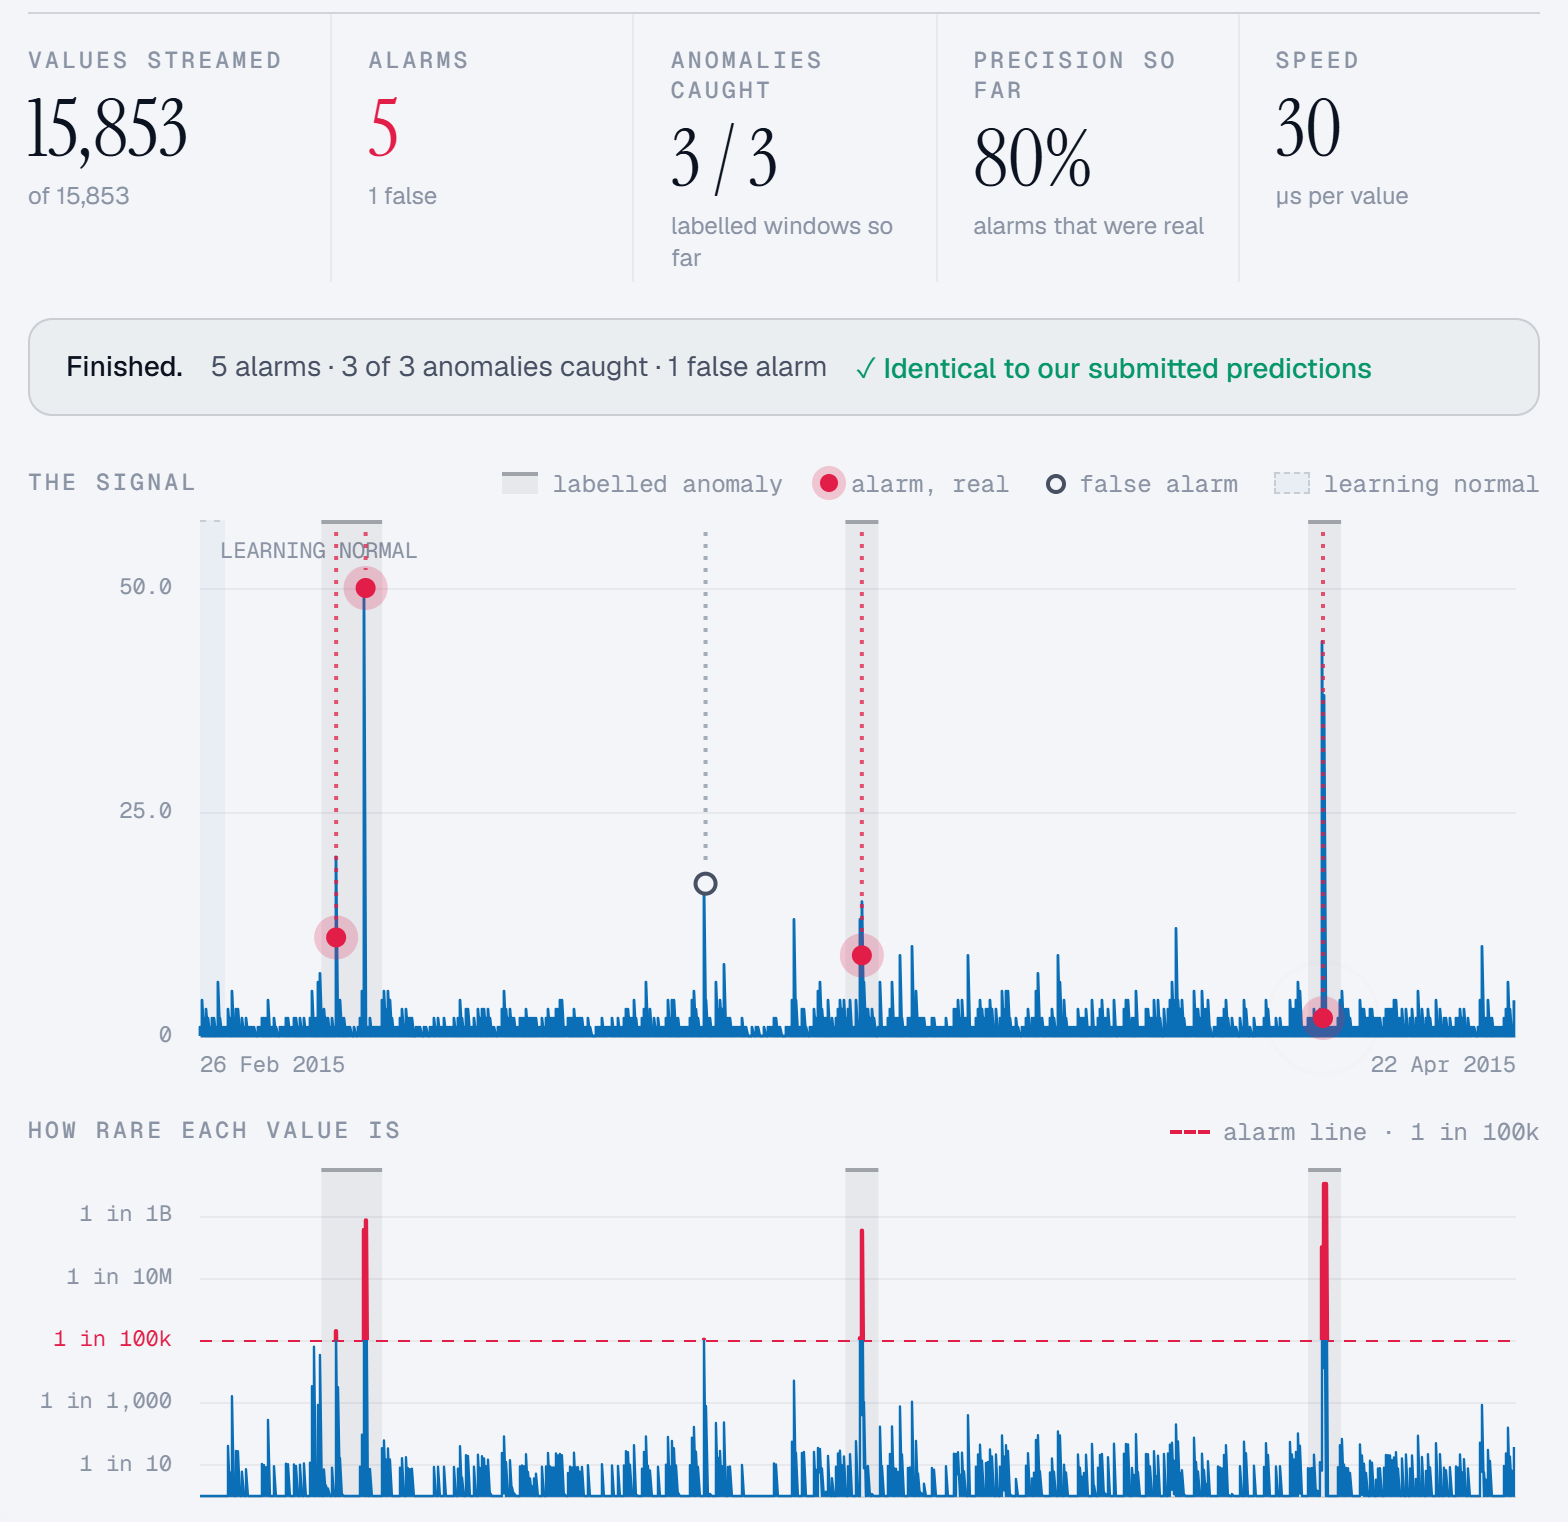
\includegraphics[width=\linewidth]{web_demo}
      \howto{our live web demo after streaming 15,853 tweet counts about CVS. Red dots: real alarms; hollow
        dot: the one false alarm.}
    \column{0.6\textwidth}
      \head{The evidence, exactly as Sentinel wrote it}
      \ev{SPIKE · 5 Mar 19:57 · score 8.5}{Value 50.00 is 99.4 scales above the learned baseline 0.32
        (normal band −1.18 to 1.82).}\par\vspace{1.2mm}
      \ev{NEW LEVEL · 26 Mar 14:07 · score 5.1}{Sustained level shift: recent mean 6.40 vs baseline 0.43
        (8.2 scales above).}\par\vspace{1.2mm}
      \ev{NEW SHAPE · 14 Apr 21:02 · score 6.0}{The last 8 points form a pattern not seen before: the closest
        past match (1,750 steps ago) differs by 11.40 per point.}\par
      \vspace{2.5mm}
      \head{Sample predictions (predictions.csv, one row per value)}
      {\scriptsize\ttfamily\setlength{\tabcolsep}{4pt}
      \begin{tabular}{@{}l r r r l l@{}}
        \toprule
        timestamp & value & score & threshold & label & watcher\\
        \midrule
        2015-03-05 19:52:53 & 0.0  & 0.000 & 5.0 & NORMAL    & \\
        2015-03-05 19:57:53 & 50.0 & 8.525 & 5.0 & \textcolor{sorange}{ANOMALOUS} & level\\
        \bottomrule
      \end{tabular}\par}
  \end{columns}
  \vfill
  \bandnote{\textbf{What this means.} An operator sees which watcher fired, how rare the value was and what normal
    looked like.}
\end{frame}

% =================================================================== 10. limits, next, conclusion
\begin{frame}{Where it still fails, why 0.594 is the ceiling for now, and the bottom line}
  \begin{columns}[T,onlytextwidth]
    \column{0.5\textwidth}
      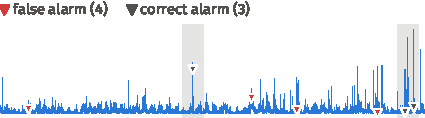
\includegraphics[width=\linewidth]{fp_example}
      \howto{tweets about IBM. Red triangles are false alarms: big bursts that nobody labelled. Most of our 39
        false alarms look like this.}
      \vspace{1.5mm}
      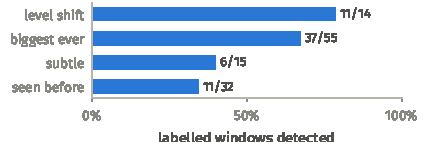
\includegraphics[width=\linewidth]{type_rates}
      \howto{share of each anomaly type that Sentinel catches. “Seen before” spikes stay hard: rarity alone
        cannot tell them from the earlier, bigger one.}
    \column{0.47\textwidth}
      \head{Why not higher than 0.594?}
      {\scriptsize\raggedright
      \textbf{Hard by nature:} 21 of the 51 misses are “seen before” spikes and 9 are subtle changes; flagging
      them would flag normal data too.\\[0.7mm]
      \textbf{Every other idea cost more than it gained:} a catch is worth about 2.4 false alarms in event-F1;
      our dropped runs paid 6 to 14. Tuning peaked at 0.594.\\[0.7mm]
      \textbf{Warm-up:} 3 anomalies start before any baseline exists.\par}
      \vspace{2mm}
      \head{Future work (needs data we do not have)}
      {\scriptsize\raggedright
      \textbf{Operator feedback:} needs people marking alarms in real use; reusing the answers would be cheating.\\[0.7mm]
      \textbf{Related signals together:} NAB gives each signal alone.\\[0.7mm]
      \textbf{Holiday effects:} no signal covers a full year, so each holiday appears at most once.\par}
      \vspace{2.5mm}
      
\begin{tikzpicture}
        \node[fill=slate, text=white, text width=\dimexpr\linewidth-12pt\relax, inner sep=5pt,
              align=left, font=\scriptsize] {\textbf{Bottom line.} Sentinel finds 65 of 116 real anomalies, 63\% of
          its alarms are correct, it runs live at 61\,µs per value, and it explains every alarm.};
      \end{tikzpicture}
  \end{columns}
\end{frame}

\end{document}
